\section{Results}
\label{sec:results}

\subsection{Data pruning}
\begin{itemize}
    \item Median response time was 15 minutes, but wide variance.
    \item Attention checks didn't work that well.
\end{itemize}

\subsection{Biases}
\begin{itemize}
    \item High-paranoia people didn't respond because our survey required
        JavaScript.
    \item Self-selection bias.
    \item We reached mostly heavy Tor users who presumably know more than the
        occasional user.
\end{itemize}

\subsection{Data quality}
\begin{itemize}
    \item Attention checks.
\end{itemize}

\subsection{Demographics}
Table~\ref{tab:survey-demo} shows the demographics of our survey.  Not
surprisingly, our demographic is \emph{young and educated}: more than sixty
percent of respondents are younger than 36, and another sixty percent has at
least a graduate degree.  Finally, another sixty percent considers themselves
at least highly knowledgeable in matters of Internet privacy and security.

\begin{figure}
\centering
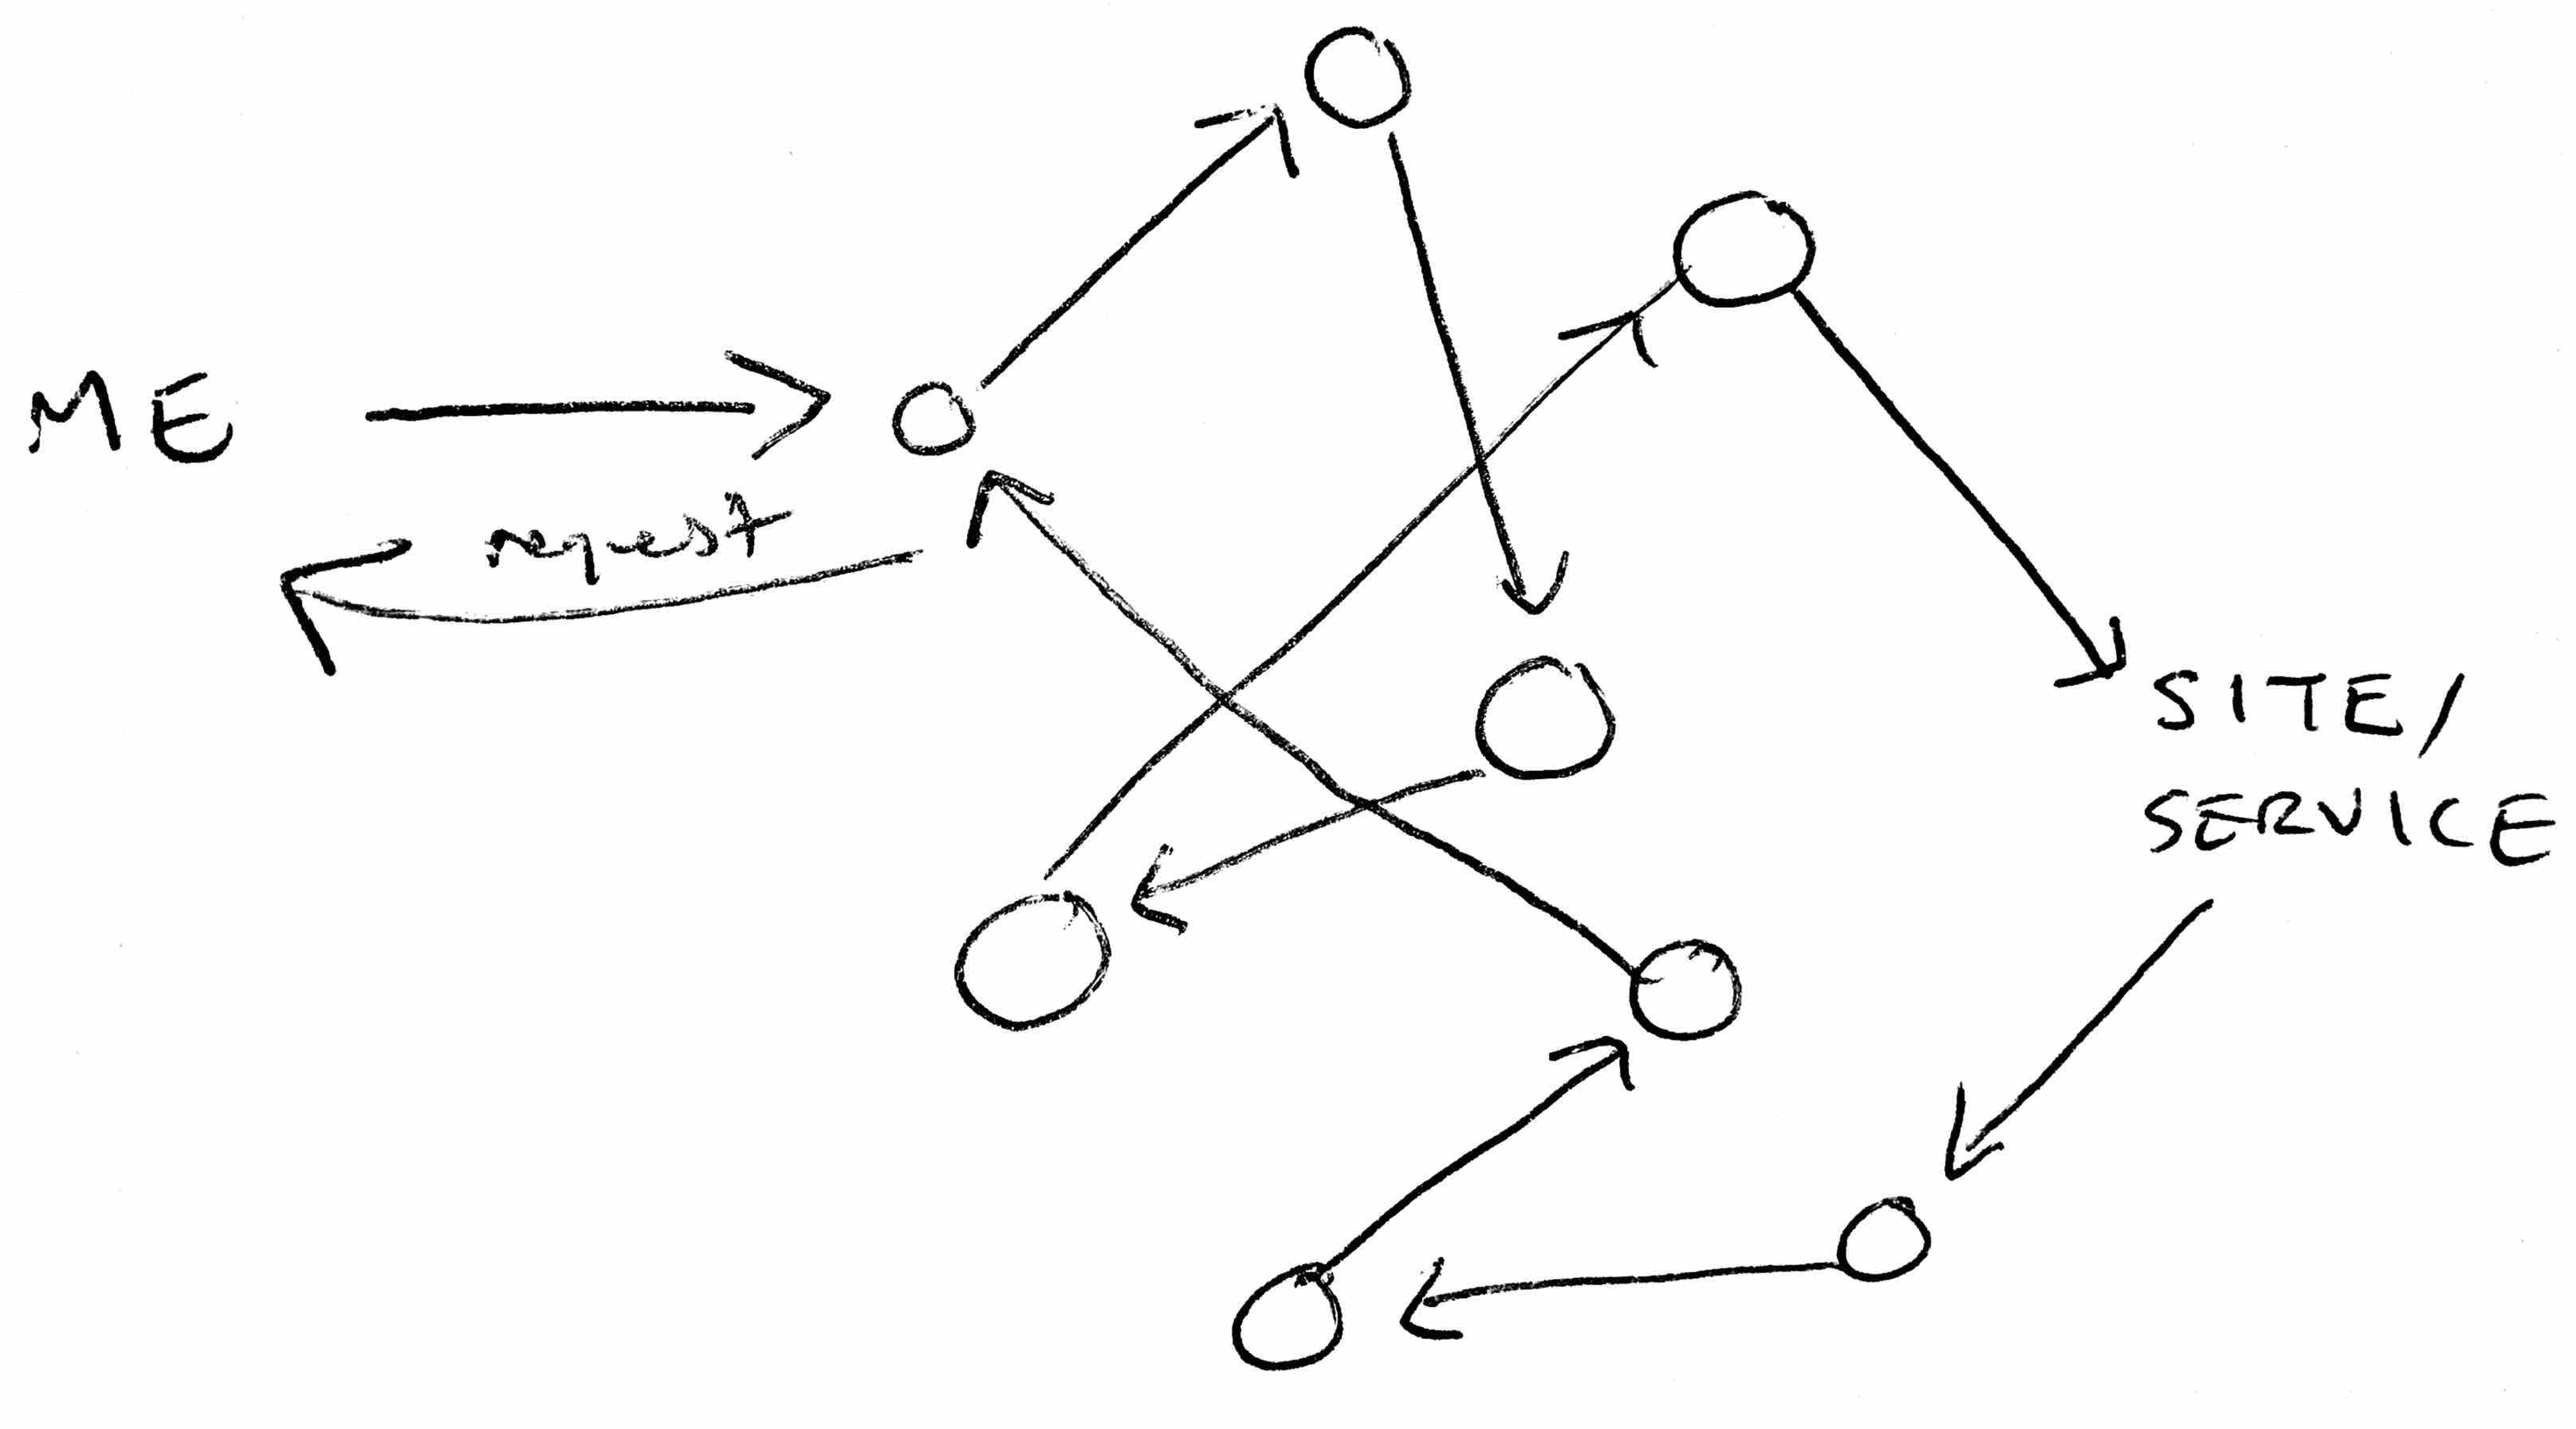
\includegraphics[width=\linewidth]{figures/p08-sketch.pdf}
\caption{Not all subjects had a correct mental model of the Tor network but
everyone understood that Tor redirects network traffic over nodes.}
\label{fig:p11-sketch}
\end{figure}

\begin{table*}[ht]
	\centering
	\begin{tabular}{l r l r l r l r}
	\toprule
	\multicolumn{2}{c}{Gender (\%)} &
	\multicolumn{2}{c}{Age (\%)} &
	\multicolumn{2}{c}{Education (\%)} &
	\multicolumn{2}{c}{Domain knowledge (\%)} \\
	\midrule
	Female & 8.9  & 18--25   & 35.5 & No degree     & 5.5  & No knowledge             & 0.5  \\
	Male   & 86.3 & 26--35   & 34.6 & High school   & 31.9 & Mildly knowledgeable     & 7.6  \\
	Other  & 4.8  & 36--45   & 17.5 & Graduate      & 42.3 & Moderately knowledgeable & 32.4 \\
	       &      & 46--55   & 8.7  & Post graduate & 20.4 & Highly knowledgeable     & 44.9 \\
	       &      & 56--65   & 2.5  &               &      & Expert                   & 14.6 \\
	       &      & $>$ 65   & 1.2  &               &      & & \\
	\bottomrule
	\end{tabular}
	\caption{The distribution over gender, age, education, and domain knowledge 
	for our 621 interview subjects.}
	\label{tab:survey-demo}
\end{table*}

\subsection{Tor usage}
The three entities most Tor users seek to protect themselves against are
governments (X\%), ISPs (X\%), and corporations (X\%).  Generally speaking,
people use Tor to protect themselves from a wide variety of threats including:
\begin{description}
    \item[Corporations] because of tracking, advertising, and profiling.  Some
        respondents specifically pointed out Google and Facebook.
    \item[Service providers] such as ISPs, backbone ISPs, and websites
        themselves.  In fact, the ISP is the most popular ``threat'' to our
        respondents with XX\%.
    \item[Governments] because of mass surveillance, law enforcement, and
        government-mandated censorship.  Governments are the second most
        popular threat with XX\%.
    \item[Personal threats] including identity theft, targeted harassment, and
        stalking.
    \item[Research] allows users to learn about a topic without revealing their
        interest in it.  Some respondents use Tor for search engine
        optimization, computer security research, and to research medical
        conditions.
    \item[Technical] use cases include IPv6 connectivity, the evasion of
        geographical restrictions, and access to onion services.  A small
        number of respondents is only interested in technical aspects other
        than privacy.
\end{description}

One respondent stated that they don't need anonymity themselves but instead use
Tor to provide cover traffic for ``people who need protection.''

Another respondent uses Tor to have IPv6 connectivity---some exit relays are
multi-homed and can connect to both IPv4 and IPv6 endpoints.

Finally, some respondents mentioned that they are using Tor only to connect to
onion services.

Half of our respondents use Tor either once a day or consider Tor Browser their
main browser.

\subsection{Onion service usage}
\subsection{Onion service operation}
\subsection{Onion service phishing}
\subsection{Expectations of privacy}

\subsection{Participants}
\begin{itemize}
    \item Provide intuition on how much our sample resembles the general
        population.
    \item From when to when did we disseminate our survey?
    \item How many participants did we attract?
    \item How long did it take to complete the survey?  Provide some descriptive statistics.
    \item What's the female/male ratio?
    \item What's the age distribution?
    \item What's the level of education?
    \item What's the computer security knowledge?  Note that our participants
        may overestimate their knowledge.
\end{itemize}

\subsection{Random anecdotes}
\begin{itemize}
    \item In pre-test: one person considered the onion domain itself
        confidential and was worried about the domain's prefix revealing
        anything about its content.
\end{itemize}
